\chapter{Hojas de estilo CSS}
% Imagen faltaaaaaaaaa    
\section{Contenidos en Parte 4}
\begin{itemize}
    \item Estilos mediante CSS
    \item Añadiendo un Icono de Aplicación
\end{itemize}
\section{Estilos mediante CSS}
En JavaFX puedes dar estilo al interfaz de usuario utilizando hojas de estilo en cascada (CSS). 
¡Esto es estupendo! Nunca había sido tan fácil personalizar la apariencia de una aplicación Java.\\
En este tutorial vamos a crear un tema oscuro (DarkTheme) inspirado en el diseño de Windows 8 Metro. 
El código CSS de los botones está basado en el artículo de blog  
\textcolor{azul}{\href{https://pixelduke.com/2012/10/23/jmetro-windows-8-controls-on-java/}{JMetro - Windows 8 Metro controls on 
Java}} por Pedro Duque Vieira.
\subsection{Familiarizándose con CSS}
Para poder aplicar estilos a una aplicación JavaFX application debes tener una comprensión básica de CSS 
en general. Un buen punto de partida es este tutorial: 
\textcolor{azul}{\href{https://www.csstutorial.net/}{CSS tutorial}}.\\
Para información más específica de CSS y JavaFX puedes consultar:
\begin{itemize}
    \item \textcolor{azul}{\href{https://docs.oracle.com/javase/8/javafx/user-interface-tutorial/css_tutorial.htm}{Skinning JavaFX Applications with CSS}} - Tutorial de Oracle
    \item \textcolor{azul}{\href{https://docs.oracle.com/javase/8/javafx/api/javafx/scene/doc-files/cssref.html}{JavaFX CSS Reference}} - Referencia oficial
\end{itemize}
\subsection{Estilo por defecto en JavaFX}
Los estilos por defecto de JavaFX 8 se encuentran en un archivo denominado \codigo{modena.css}. 
Este archivo CSS se encuentra dentro del archivo jar \codigo{jfxrt.jar} que se encuentra en tu 
directorio de instalación de Java, en la ruta \codigo{/jdk1.8.x/jre/lib/ext/jfxrt.jar}.\\
Puedes descomprimir \codigo{jfxrt.jar} o abrirlo como si fuera un zip. Encontrarás el archivo 
\codigo{modena.css} en la ruta \codigo{com/sun/javafx/scene/control/skin/modena/}\\
Este estilo se aplica siempre a una aplicación JavaFX. Añadiendo un estilo personal 
podemos reescribir los estilos por defecto definidos en \codigo{modena.css}.

\begin{tcolorbox}[leftrule=3mm]
	\textbf{Truco:} Ayuda consultar el archivo CSS por defecto para ver qué estilos necesitas sobreescribir.
\end{tcolorbox}
\subsection{Vinculando hojas de estilo CSS}
Añade un archivo CSS denominado \codigo{DarkTheme.css} al paquete \textit{view}.\\
\codigo{DarkTheme.css}
\begin{minted}[
    linenos,
    numbersep=5pt,
    gobble=0,
    frame=lines,
    framesep=2mm,
    breaklines=true,
    ]{css}
    .background {
    -fx-background-color: #1d1d1d;
}

.label {
    -fx-font-size: 11pt;
    -fx-font-family: "Segoe UI Semibold";
    -fx-text-fill: white;
    -fx-opacity: 0.6;
}

.label-bright {
    -fx-font-size: 11pt;
    -fx-font-family: "Segoe UI Semibold";
    -fx-text-fill: white;
    -fx-opacity: 1;
}

.label-header {
    -fx-font-size: 32pt;
    -fx-font-family: "Segoe UI Light";
    -fx-text-fill: white;
    -fx-opacity: 1;
}

.table-view {
    -fx-base: #1d1d1d;
    -fx-control-inner-background: #1d1d1d;
    -fx-background-color: #1d1d1d;
    -fx-table-cell-border-color: transparent;
    -fx-table-header-border-color: transparent;
    -fx-padding: 5;
}

.table-view .column-header-background {
    -fx-background-color: transparent;
}

.table-view .column-header, .table-view .filler {
    -fx-size: 35;
    -fx-border-width: 0 0 1 0;
    -fx-background-color: transparent;
    -fx-border-color:
        transparent
        transparent
        derive(-fx-base, 80%)
        transparent;
    -fx-border-insets: 0 10 1 0;
}

.table-view .column-header .label {
    -fx-font-size: 20pt;
    -fx-font-family: "Segoe UI Light";
    -fx-text-fill: white;
    -fx-alignment: center-left;
    -fx-opacity: 1;
}

.table-view:focused .table-row-cell:filled:focused:selected {
    -fx-background-color: -fx-focus-color;
}

.split-pane:horizontal > .split-pane-divider {
    -fx-border-color: transparent #1d1d1d transparent #1d1d1d;
    -fx-background-color: transparent, derive(#1d1d1d,20%);
}

.split-pane {
    -fx-padding: 1 0 0 0;
}

.menu-bar {
    -fx-background-color: derive(#1d1d1d,20%);
}

.context-menu {
    -fx-background-color: derive(#1d1d1d,50%);
}

.menu-bar .label {
    -fx-font-size: 14pt;
    -fx-font-family: "Segoe UI Light";
    -fx-text-fill: white;
    -fx-opacity: 0.9;
}

.menu .left-container {
	-fx-background-color: black;
}

.text-field {
    -fx-font-size: 12pt;
    -fx-font-family: "Segoe UI Semibold";
}

/*
 * Metro style Push Button
 * Author: Pedro Duque Vieira
 * http://pixelduke.wordpress.com/2012/10/23/jmetro-windows-8-controls-on-java/
 */
.button {
    -fx-padding: 5 22 5 22;
    -fx-border-color: #e2e2e2;
    -fx-border-width: 2;
    -fx-background-radius: 0;
    -fx-background-color: #1d1d1d;
    -fx-font-family: "Segoe UI", Helvetica, Arial, sans-serif;
    -fx-font-size: 11pt;
    -fx-text-fill: #d8d8d8;
    -fx-background-insets: 0 0 0 0, 0, 1, 2;
}

.button:hover {
    -fx-background-color: #3a3a3a;
}

.button:pressed, .button:default:hover:pressed {
  -fx-background-color: white;
  -fx-text-fill: #1d1d1d;
}

.button:focused {
    -fx-border-color: white, white;
    -fx-border-width: 1, 1;
    -fx-border-style: solid, segments(1, 1);
    -fx-border-radius: 0, 0;
    -fx-border-insets: 1 1 1 1, 0;
}

.button:disabled, .button:default:disabled {
    -fx-opacity: 0.4;
    -fx-background-color: #1d1d1d;
    -fx-text-fill: white;
}

.button:default {
    -fx-background-color: -fx-focus-color;
    -fx-text-fill: #ffffff;
}

.button:default:hover {
    -fx-background-color: derive(-fx-focus-color,30%);
}
\end{minted}
A continuación, necesitamos vincular el CSS a nuestra escena. Podemos hacer esto programáticamente, 
mediante código Java, pero en esta ocasión vamos a utilizar \textit{Scene Builder} para añadirlo a 
nuestros archivos FXML:\\
\subsubsection*{Añade el CSS a RootLayout.fxml}
\begin{enumerate}
    \item Abre el archivo \codigo{RootLayout.fxml} en \textit{Scene Builder}.
    \item Selecciona el \codigo{BorderPane} raíz en la sección \textit{Hiperarchy}. En la vista \textit{Properties} añade 
    el archivo \codigo{DarkTheme.css} como hoja de estilo (campo denominado \codigo{Stylesheets}).
    \begin{figure}[H]
        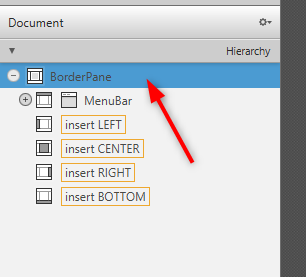
\includegraphics{img/6-1-Hierachy.png}
    \end{figure}
    \begin{figure}[H]
        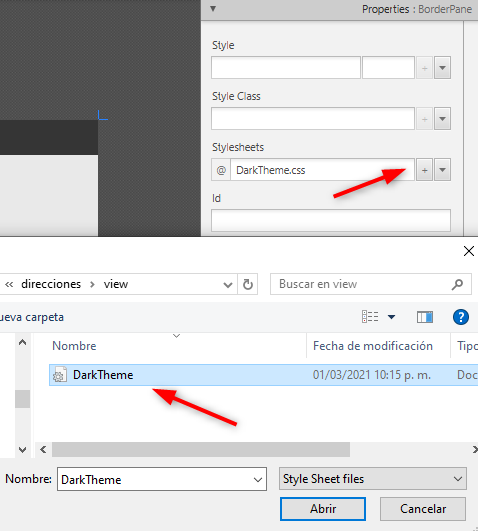
\includegraphics{img/6-2-SelectCSS.png}
    \end{figure}
\end{enumerate}

\subsubsection*{Añade el CSS a PersonEditDialog.fxml}
\begin{enumerate}
    \item Abre el archivo \codigo{PersonEditDialog.fxml} en \textit{Scene Builder}. Selecciona el \codigo{AnchorPane} 
    raíz e incluye \codigo{DarkTheme.css} como hoja de estilo en la sección \textit{Properties}.
    \begin{figure}[H]
        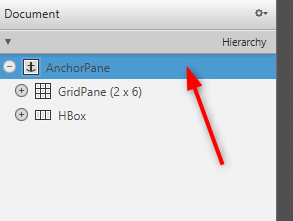
\includegraphics{img/6-3-SelectAnchorPane.png}
    \end{figure}
    \item El fondo todavía es blanco, hay que añadir la clase \codigo{background} al \codigo{AnchorPane} raíz.
    \begin{figure}[H]
        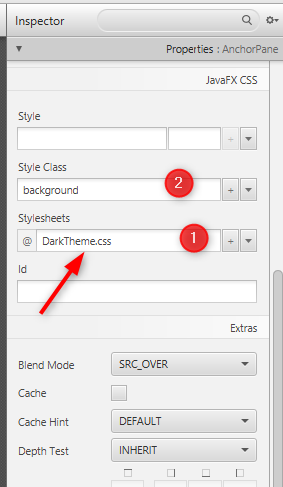
\includegraphics{img/6-4-AddCSS.png}
    \end{figure}
    \item Selecciona el botón OK y elige \textit{Default Button} en la vista \textit{Properties}. Eso cambiará su 
    color y lo convertirá en el botón “por defecto”, el que se ejecutará si el usuario aprieta la tecla \textit{enter}.
\end{enumerate}
\subsubsection*{Añade el CSS a PersonOverview.fxml}
\begin{enumerate}
    \item Abre el archivo \codigo{PersonOverview.fxml} en \textit{Scene Builder}. Selecciona el \codigo{AnchorPane} raíz 
    en la sección \textit{Hierarchy} y añade \codigo{DarkTheme.css} a sus \codigo{Stylesheets}.
    \begin{figure}[H]
        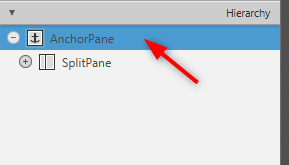
\includegraphics{img/6-5-AnchorPane.png}
    \end{figure}
    \begin{figure}[H]
        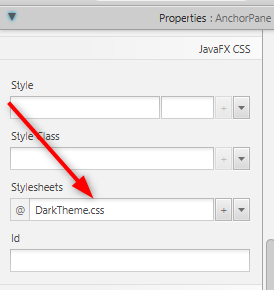
\includegraphics{img/6-6-SelectDark.png}
    \end{figure}
    \item A estas alturas deberías haber observado algunos cambios: La tabla y los botones son negros. 
    Las clases de estilo \codigo{.table-view} y \codigo{.button} de \codigo{modena.css} se aplican automáticamente a la tabla y 
    los botones. Ya que hemos redefinido (sobreescrito) algunos de esos estilos en nuestro propio CSS, 
    los nuevos estilos se aplican automáticamente.
    \item Posiblemente tengas que ajustar el tamaño de los botones para que se muestre todo el texto.
    \item Selecciona el panel \codigo{AnchorPane} de la derecha, dentro del \codigo{SplitPane}.
    \begin{figure}[H]
        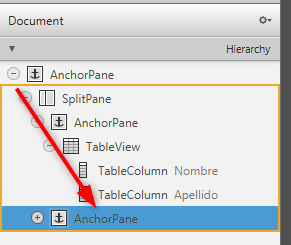
\includegraphics{img/6-7-AnchorPane.png}
    \end{figure}
    \item Ves a la vista \textit{Properties} y elige \codigo{background} como clase de estilo. 
    El fondo debería volverse negro.
    \begin{figure}[H]
        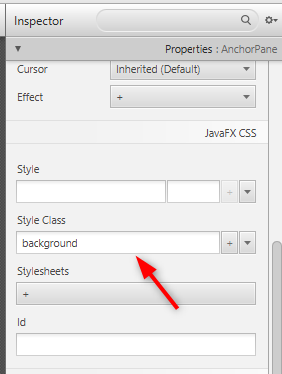
\includegraphics{img/6-8-BackGround.png}
    \end{figure}
\end{enumerate}

\subsubsection*{Etiquetas con un estilo diferente}
En este momento, todas las etiquetas en el lado derecho tienen el mismo tamaño. 
Ya tenemos definidos en el CSS unos estilos denominados \codigo{.label-header} y \codigo{.label-bright} 
que vamos a usar para personalizar la apariencia de las etiquetas.
\begin{enumerate}
    \item Selecciona la etiqueta (\codigo{Label}) \textit{Detalle de personas} y añade \codigo{label-header} 
    como clase de estilo.
    \begin{figure}[H]
        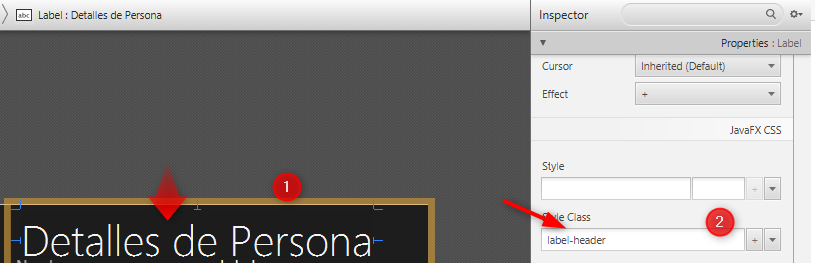
\includegraphics{img/6-9-DetallePerson.png}
    \end{figure}
    \item A cada etiqueta en la columna de la derecha (donde se muestran los detalles 
    de una persona), añade la clase de estilo \codigo{label-bright}.
    \begin{figure}[H]
        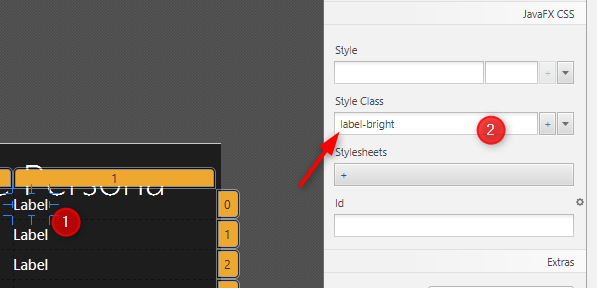
\includegraphics{img/6-10-labelBright.png}
    \end{figure}
\end{enumerate}

\section{Añadiendo un icono a la aplicación}
Ahora mismo nuestra aplicación utiliza el icono por defecto para la barra de título y la barra de tareas:\\
Quedaría mucho mejor con un icono propio:\\
\begin{figure}[H]
	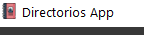
\includegraphics[width=11cm]{img/6-11-icono.png}
\end{figure}
\subsection{El archivo de icono}
Un posible sitio para obtener iconos gratuitos es \textcolor{azul}{\href{https://www.iconfinder.com/}{Icon Finder}}. %Revisar, ya no existe la página
Yo por ejemplo descargué este icono de libreta de direcciones.\\
Crea una carpeta dentro de tu aplicación llamado \textbf{resources} y añádele una subcarpeta 
para almacenar imágenes, llámala \textbf{images}. Pon el icono que hayas elegido dentro de la 
carpeta de imágenes. La estructura de directorios de tu carpeta debe tener un aspecto similar a este:
\begin{figure}[H]
	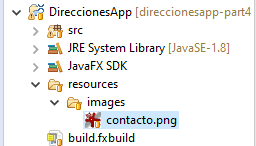
\includegraphics[width=11cm]{img/6-12-selectIcon.png}
\end{figure}
\subsection{Establece el icono de la escena principal}
Para establecer el icono de nuestra escena debemos añadir la línea de 
código siguiente al método \codigo{start(...)} dentro de \codigo{MainApp.java}.\\
\codigo{MainApp.java}\\
Código
\begin{minted}[
    linenos,
    numbersep=5pt,
    gobble=0,
    frame=lines,
    framesep=2mm,
    breaklines=true,
    ]{java}
    //Colocar el icono
	this.primaryStage.getIcons().add(new Image("file:resources/images/contacto.png"));
\end{minted}
El método \codigo{start(...)} debería verse así ahora:\\
Código
\begin{minted}[
    linenos,
    numbersep=5pt,
    gobble=0,
    frame=lines,
    framesep=2mm,
    breaklines=true,
    ]{java}
    public void start(Stage primaryStage) {
		this.primaryStage = primaryStage;
		this.primaryStage.setTitle("Directorios App");

		initRootLayout();
		showPersonaOverview();

		//Colocar el icono
		this.primaryStage.getIcons().add(new Image("file:resources/images/contacto.png"));
	}
\end{minted}
También puedes añadir un icono a la escena que contiene la venta de edición de los detalles de una persona.